\chapter{Estudos de Caso}
\label{cap:estudo}

A replicação ativa permite a construção de aplicações que compartilham dados entre suas instâncias, sem que seja necessário centralizar essas informações. Em uma aplicação replicada, cada instância possui uma cópia de todos os dados do sistema. Cada instância é uma réplica das demais, e funciona como um histórico das ações realizadas pelo sistema.

Jogos de tabuleiro são exemplos de aplicações que podem ser implementadas usando replicação. Esses jogos possuem diversos elementos e informações que precisam ser compartilhadas entre seus jogadores, como o tabuleiro, as peças, a posição de cada peça, a situação atual da partida. Nesse caso a replicação permite que jogadores usando instâncias diferentes da aplicação compartilhem esses elementos e informações. Esse estudo de caso mostra a implementação de um jogo de tabuleiro, usando Treplica, metaobjetos, e Cyan, no intuito de demonstrar como o uso da metaprogramação permite implementar aplicações replicadas de modo transparente.

Em seguida é mostrada uma aplicação exemplo que, durante a compilação, tem seus métodos não deterministas trocados por métodos deterministas. Para facilitar a demonstração da mecânica de substituição dos métodos foram usados métodos deterministas para representar os métodos não deterministas. Assim, foi possível definir nomes significativos para os métodos do exemplo. Trechos do código-fonte e o arquivo \emph{deterministic} dessa aplicação são mostrados na Sessão~\ref{sec:estudodtcomp}.

\section{Disputa pela Rota do Leste}

O jogo de tabuleiro Disputa pela Rota do Leste é uma batalha entre guerreiros e magos que estão disputando uma rota comercial com os reinos do leste. Ele é uma aplicação desenvolvida em Cyan que deve ser usada por dois jogadores, cada um com uma instância diferente do programa. As instâncias de cada jogador podem ser executadas no mesmo computador, para simplificar a demonstração.

Cada jogador controla um grupo três personagens (dois guerreiros e um mago) e o jogo é baseado em rodadas e ações. Em cada rodada um determinado jogador pode realizar três ações de ataque e movimento. A ação de selecionar personagens pode ser realizada sem limitação durante a rodada. A ação \emph{START} reinicia a partida. Os jogadores não podem executar ações durante a rodada do oponente, e após realizar três ações, a vez é passada para o oponente. Todas as ações são realizadas via um terminal de texto, que recebe os comandos dos jogadores. O jogo termina quando todos os personagens de um jogador estiverem fora de combate.

A Figura~\ref{fig:Tabuleiro} mostra uma instância da aplicação sendo executada. À esquerda é representado o tabuleiro, que é definido pelos símbolos: \srcstyle{.}, \srcstyle{?}, \srcstyle{@}, \srcstyle{\#}. O ponto (\srcstyle{.}) representa os espaços por onde os personagens podem se mover. O ponto de interrogação (\srcstyle{?}) representa o mago, e o guerreiro é representado pela arroba (\srcstyle{@}). Os obstáculos são representadas no tabuleiro pelo cardinal (\srcstyle{\#}), os personagens não podem se mover passando por eles.

À direita são representadas as informações referentes à partida. São mostrados os jogadores (\srcstyle{Player}), os personagens e suas vidas (\srcstyle{Mage 1}), os pontos de ação disponíveis para a rodada (\srcstyle{Action Points}), e qual o personagem selecionado (\srcstyle{Selected}). As informações correspondentes ao jogador associado à instância da aplicação estão em - \srcstyle{Player 1} - \srcstyle{YOU}, as informações em - \srcstyle{Player 2} - \srcstyle{OPONENT} - são referentes ao jogador que está usando a outra instância da aplicação.

\begin{figure}[H]
	\centering
	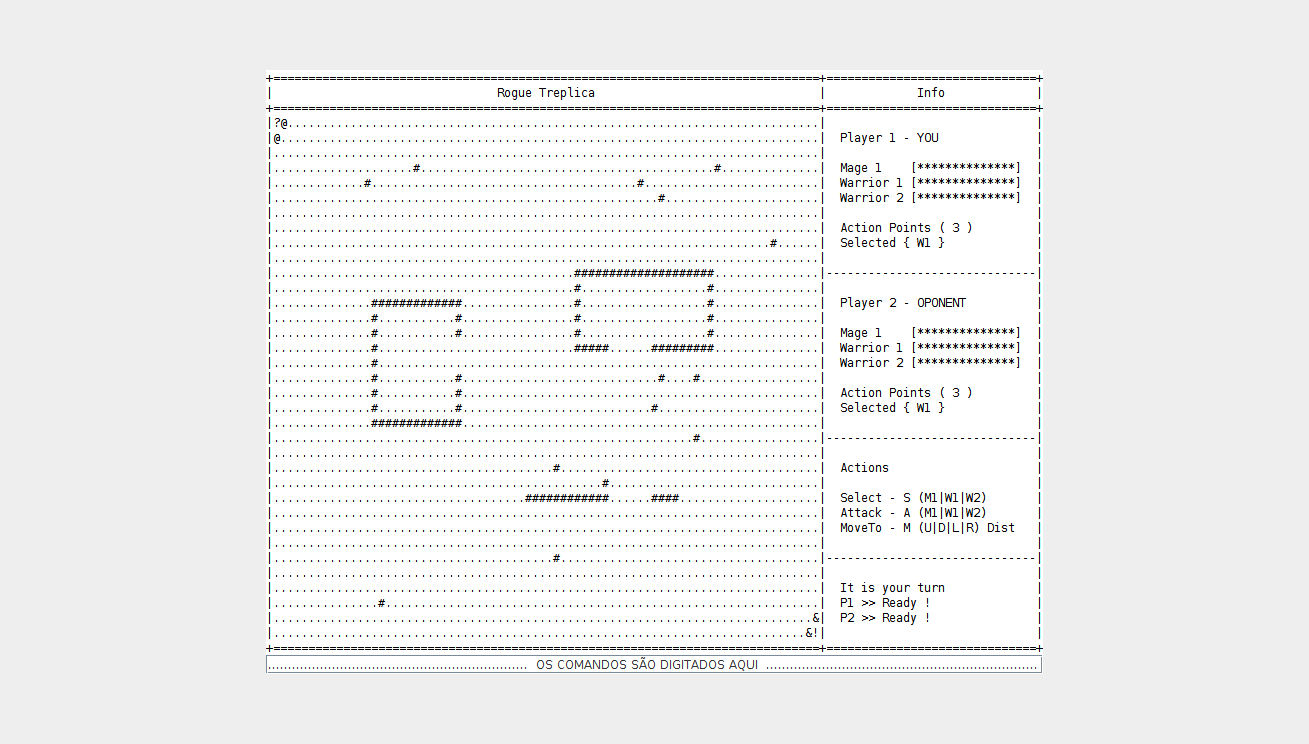
\includegraphics[trim={9.38cm 2.45cm 9.38cm 2.5cm},clip,scale=0.57]{conteudo/capitulos/figs/tabuleiro.png}
	\caption{Uma instância da aplicação sendo executada}
	\label{fig:Tabuleiro}
\end{figure}

Ainda à direita da figura, a seção \srcstyle{Actions} mostra como os jogadores devem construir os comandos. A ação de selecionar personagens , \srcstyle{Select}; é formada pela letra \srcstyle{S} seguida do personagem a ser selecionado ( \srcstyle{M1}: mago, \srcstyle{W1} e \srcstyle{W2}: guerreiros). A ação \srcstyle{Attack} é usada para atacar um personagem do oponente, ela é formada pela letra \srcstyle{A} seguida do personagem pertencente ao oponente que será atacado, caso o atacante esteja distante do seu alvo o ataque não ocorrerá. 

A última ação disponível é a \srcstyle{MoveTo}, usada para mover um personagem pelo tabuleiro, ela é formada pela letra \srcstyle{M} seguida da direção que o personagem irá se mover (\srcstyle{U}: cima, \srcstyle{D}: baixo, \srcstyle{L}: esquerda, \srcstyle{R}: direita), e da distância que ele irá se deslocar (número de espaços).  Caso o movimento não possa ocorrer por causa de um obstáculo ou por causa da distância, uma mensagem será exibida. As ações são realizadas com base no personagem selecionado, é ele quem se movimenta e ataca.

A última seção à direita mostra se a rodada atual pertence ao jogador dessa instância da aplicação (\srcstyle{It is your turn}). Essa seção também exibe a última atualização associada a cada jogador (\srcstyle{P1 >> Ready!}), pode mostrar mensagens de alerta, e indicar o resultado das ações desse jogador. Os comandos são digitados pelos jogadores no espaço abaixo do tabuleiro e das informações, no local indicado na Figura~\ref{fig:Tabuleiro}.

\subsection{Implementação do Protótipo de um Tabuleiro Compartilhado}

Para implementar esse jogo de tabuleiro foram desenvolvidos quatorze protótipos. O protótipo \srcstyle{Board} é de maior importância. Ele é quem define o contexto (\srcstyle{Context}) e as ações (\srcstyle{Action}) de Treplica. Os outros protótipos são usados para separar os elementos da aplicação e tornar o código melhor organizado. Podemos considerar o protótipo \srcstyle{Board} como o centro da aplicação, pois ele é quem acaba integrando os outros protótipos. 

O protótipo \srcstyle{Entity} (Código-Fonte~\ref{cod:RogueEntity}) define dois métodos: o método \srcstyle{getType}, que retorna o tipo da entidade, e o método \srcstyle{draw} usado para desenhar a entidade no mapa. Esse protótipo é herdado pelos protótipos \srcstyle{Figure} e \srcstyle{Tile} que sobrescrevem seus métodos. Desse modo o protótipo \srcstyle{Map} pode usar os métodos de \srcstyle{Entity} para acessar tanto as instâncias de \srcstyle{Figure}, como de \srcstyle{Tile}. Isso permite que o protótipo \srcstyle{Map} mantenha uma única matriz do tipo \srcstyle{Entity} contendo instâncias de ambos os protótipos.

\begin{lstlisting}[language=Java, caption={Protótipo \textbf{Entity} herdado por \emph{Figure} e \emph{Tile}}, label={cod:RogueEntity}]
package main

object Entity
  func getType -> Int { return Const ENTITY; }
  func draw { }
end
\end{lstlisting}

O protótipo \srcstyle{Figure} representa uma peça do tabuleiro, um mago ou um guerreiro. Ele possui métodos como \srcstyle{setPosition} para marcar a posição da peça no mapa, \srcstyle{setLife} para modificar os pontos de vida da peça quando ela é atacada, \srcstyle{getDistanceMax} para verificar a distância máxima que a peça pode ser deslocada com um movimento. Os elementos que compõem o cenário como o chão e os obstáculos por sua vez são representados pelo protótipo \srcstyle{Tile}. Métodos como \srcstyle{draw} e \srcstyle{getType} são implementados por ambos os protótipos, \srcstyle{Figure} e \srcstyle{Tile}, uma vez que eles herdam de \srcstyle{Entity}.

O mapa com todas as peças e partes do cenário é mantido pelo protótipo \srcstyle{Board} como parte do contexto de Treplica, definido o estado a ser replicado. O protótipo \srcstyle{Board} mantém um vetor de instâncias do tipo \srcstyle{Player} e a variável \srcstyle{currentPlayer}, que é uma referência para o \srcstyle{Player} que tem direito a jogar na rodada atual. O protótipo \srcstyle{Board} define quatro ações de Treplica: \srcstyle{startAction}, chamada para reiniciar o jogo; \srcstyle{moveAction}, usada pelos jogadores para mover as peças pelo mapa; \srcstyle{attackAction}, chamada para que uma peça ataque um mago ou guerreiro inimigo; e \srcstyle{selectAction}, que permite aos jogadores selecionarem qual peça eles querem que se mova ou ataque. O Código-Fonte~\ref{cod:RogueBoard} mostra a implementação parcial do protótipo \srcstyle{Board} que usa a anotação do metaobjeto \srcstyle{@treplicaAction} para marcar os métodos que serão as ações de Treplica.

\begin{lstlisting}[language=Java, caption={Protótipo \textbf{Board} que integra a aplicação}, label={cod:RogueBoard}]
package main

import treplica
import cyan.math

object Board extends Context
  var Map map
  var Array< Player > players
  var String currentPlayer
  ...
  @treplicaAction
  func selectAction: String target { ... }

  @treplicaAction
  func attackAction: String target { ... }

  @treplicaAction
  func moveAction: String direction, String value { ... }
  ...
  @treplicaAction
  func startAction { ... }
  ...
end
\end{lstlisting}

Não se pode deixar de mencionar o protótipo \srcstyle{Program} mostrado no Código-Fonte~\ref{cod:RogueProgMain}. Ele usa a anotação do metaobjeto \srcstyle{@treplicaInit} para iniciar a máquina de estados de Treplica e implementa o método \srcstyle{event}, que recebe os comandos dos jogadores e chama os métodos replicados do contexto. 

O \emph{loop} principal da aplicação está implementado no protótipo \srcstyle{Window}. Esse protótipo aguarda comandos do jogador na forma de entrada via teclado (comando) e chama o método \srcstyle{event} de \srcstyle{Program} passando essa entrada. Note que os métodos de \srcstyle{local} que representam ações de Treplica também são chamados pela sua máquina de estados. Em ambos os casos a tela do jogo é atualizada após cada chamada de uma ação. Alguns protótipos usados para implementar essa aplicação não foram detalhados por não serem relevantes para a compreensão da implementação desse estudo de caso.

\begin{lstlisting}[language=Java, caption={Protótipo \textbf{Program} do Jogo de Tabuleiro}, label={cod:RogueProgMain}]
package main
import treplica

object Program extends Input
  ...
  override func event: String text {
    ...
    local selectAction: temp1;
    ...
    local attackAction: temp1;
    ...
    local moveAction: temp1, temp2;
    ...
  }

  func run: Array<String> args {
    Window build: self;
    
    var local = ("/var/tmp/magic" ++ args[1]);
    @treplicaInit( 2, 200, local )
    var data = Board new: args[1];
    data startBoard;
    ...
  }
end
\end{lstlisting}

\section{Somente os Métodos Deterministas Compilaram}
\label{sec:estudodtcomp}

As aplicações replicadas baseadas em máquinas de estado têm como uma de suas principais características o determinismo de suas ações. Uma ação que será replicada deve ser determinista, caso seu comportamento fuja a essa regra ela pode tornar a aplicação inconsistente.

O metaobjeto \srcstyle{treplicaAction} é responsável por transformar métodos tradicionais em ações de Treplica e por verificar se esses métodos apresentam algum caso de não determinismo cadastrado. Nesse estudo de caso é definida uma ação de Treplica, que possui um método cadastrado como não determinista, para demonstrar como a compilação dessa aplicação localiza e trata essa inconsistência.

Essa aplicação é composta de dois protótipos. Um é similar ao protótipo definido no Código-Fonte~\ref{cod:TreplicaMainMeta} que inicializa a máquina de estados de Treplica. O outro é o protótipo do Código-Fonte~\ref{cod:NdContextExample}, que contém o contexto associado a essa máquina de estados e à ação não determinista implementada pelo método \srcstyle{nondeterministic}.

\begin{lstlisting}[language=Java, caption={Contexto com ação não determinista}, label={cod:NdContextExample}]
package main

import treplica
import cyan.math

object Tested extends Context
  var String result 
  func init { result = "hello"; }

  @treplicaAction
  func perform {
    nondeterministic: (setResult: "bye");
    Out println: "perform: " ++ self.result;
  }

  func setResult: String value -> String {
    self.result = value;
    return value;
  }

  func nondeterministic: String value {
    Out println: "nondeterministic: " ++ value ++ " random: " ++ Math random;
  }
end
\end{lstlisting}

Para que o método \srcstyle{nondeterministic} seja reconhecido como não determinista, deve ser cadastrado no arquivo \emph{deterministic} da biblioteca Treplica de Cyan ou no arquivo \emph{deterministic} da própria aplicação. Nessa caso o cadastro do método está no pacote de Treplica, como mostrado no Código-Fonte~\ref{cod:NdContextExampleRule}. Essa regra define que o método \srcstyle{nondeterministic} do protótipo \srcstyle{Tested} deve ser substituído pelo método \srcstyle{testok} do protótipo \srcstyle{Deterministic}. O método que substitui o caso não determinista deve ter os mesmos parâmetros do método substituído.

\begin{lstlisting}[language=Java, caption={Regra de substituição cadastrada}, label={cod:NdContextExampleRule}]
main,Tested,nondeterministic-treplica,Deterministic,testok
\end{lstlisting}

Dessa forma, durante a compilação o método \srcstyle{nondeterministic} será substituído pelo método \srcstyle{testok}, e a ocorrência de não determinismo será removida pelo metaobjeto \srcstyle{treplicaAction}. A compilação também emite um alerta ao desenvolvedor a respeito do não determinismo que foi substituído. Caso o protótipo ou o método que remove o não determinismo não seja encontrado, a compilação falhará. Nesses casos um erro de compilação é mostrado como resultado.

O protótipo \srcstyle{Deterministic} é mostrado no Código-Fonte~\ref{cod:NdDeterministMethodExample}. O método \srcstyle{testok} implementado possui os mesmos parâmetros do método \srcstyle{nondeterministic} e a chamada ao método \srcstyle{random} do protótipo \srcstyle{Math} foi substituída pela \emph{string} \srcstyle{23}. O método realmente não determinista é o \srcstyle{random}, ele poderia ter sido substituído diretamente, como no exemplo da sessão~\ref{sec:trcyndmeta}. Para mostrar a substituição de um método com parâmetros foi necessário encapsular o método não determinista dentro do método \srcstyle{nondeterministic}.

\begin{lstlisting}[language=Java, caption={Protótipo com método determinista}, label={cod:NdDeterministMethodExample}]
package treplica

object Deterministic

  func random -> Double {
    return 23.0;
  }

  func testok: String value {
    Out println: "testok: " ++ value ++ " random: " ++ "23";
  }
end
\end{lstlisting}

Se o método \srcstyle{random} do protótipo \srcstyle{Math} fosse substituído diretamente pelo método \srcstyle{random} do protótipo \srcstyle{Deterministic}, a regra cadastrada seria igual à mostrada no Código-Fonte~\ref{cod:NdDiretoRandomRule}, e nesse caso não existem parâmetros a serem passados ao novo método. Os protótipos implementados para remover o não determinismo devem pertencer aos pacotes \srcstyle{treplica} ou \srcstyle{main}. O metaobjeto \srcstyle{treplicaAction} pode ser melhorado para que esses protótipos possam pertencer a qualquer pacote.

\begin{lstlisting}[language=Java, caption={Regra de substituição cadastrada}, label={cod:NdDiretoRandomRule}]
cyan.math,Math,random-treplica,Deterministic,random
\end{lstlisting}

Repare que, no caso da primeira regra, a busca por métodos não deterministas inicia no método \srcstyle{perform} e termina após substituir o método \srcstyle{nondeterministic}. No caso da segunda regra, a busca se propaga recursivamente aos métodos internos do método inicial. Essa segunda busca percorre o método \srcstyle{perform} onde encontra o método \srcstyle{nondeterministic}, esse método encontrado também é percorrido na procura do método \srcstyle{random} do protótipo \srcstyle{Math}. Se a chamada de método que for substituída possuir parâmetros, esses serão mantidos na chamada do novo método.